\documentclass[conference]{IEEEtran}
\usepackage{iftex}
\ifXeTeX
  \usepackage{fontspec}
  \setmainfont{texgyretermes}[Extension=.otf, UprightFont=*-regular, BoldFont=*-bold, ItalicFont=*-italic, BoldItalicFont=*-bolditalic]
\else
  \usepackage[T1]{fontenc}
\fi
\usepackage{booktabs}
\usepackage{array}
\usepackage{amsmath}
\usepackage{tikz}
\usetikzlibrary{arrows.meta,positioning}
\usepackage[hidelinks]{hyperref}
\usepackage{url}
\urlstyle{tt}
\newcommand{\attackCalm}{33 of 180}
\newcommand{\attackGuard}{15 of 180}
\newcommand{\backboneFlows}{1,648,523}
\newcommand{\backboneHosts}{77,230}
\newcommand{\backboneKnown}{7.79\%}
\newcommand{\backboneLab}{98.3\%}
\newcommand{\backboneLocal}{0.613\%}
\newcommand{\backboneScored}{300,002}
\newcommand{\backboneScoredHosts}{41,657}
\newcommand{\backboneSpeed}{2,040}
\newcommand{\botnetRecall}{0.8\%}
\newcommand{\clearBoth}{2.0\%}
\newcommand{\clearFast}{2.7\%}
\newcommand{\clearHigh}{4.3\%}
\newcommand{\clearLow}{0.9\%}
\newcommand{\clearShare}{67\%}
\newcommand{\clearSize}{300}
\newcommand{\crossFAHigh}{64\%}
\newcommand{\crossFALow}{9\%}
\newcommand{\crossRecallHigh}{47.7\%}
\newcommand{\crossRecallLow}{0.0\%}
\newcommand{\demoOthersPassed}{11}
\newcommand{\disguiseCount}{30}
\newcommand{\disguiseHarmless}{18}
\newcommand{\eitherFA}{1.13\%}
\newcommand{\eitherRecall}{99.76\%}
\newcommand{\fakeFinalCaught}{39/44}
\newcommand{\fakeFinalWrong}{0/22}
\newcommand{\fakeLinkCaught}{40/44}
\newcommand{\fakeLinkWrong}{4/22}
\newcommand{\fakeOldCaught}{42/44}
\newcommand{\fakeOldWrong}{0/22}
\newcommand{\fastHarmful}{68.7\%}
\newcommand{\fastHarmfulSilent}{36}
\newcommand{\fastSystemBlocked}{13}
\newcommand{\fastSystemFA}{17.3\%}
\newcommand{\fastSystemMedian}{0.11}
\newcommand{\fastSystemPrecision}{93.9\%}
\newcommand{\fastSystemRecall}{89.6\%}
\newcommand{\finalLater}{0.995}
\newcommand{\firstRunBlocked}{25}
\newcommand{\firstRunClean}{150}
\newcommand{\firstRunCleanFA}{19.3\%}
\newcommand{\firstRunHandWrong}{1 of 21}
\newcommand{\firstRunOpinionWrong}{19/22}
\newcommand{\firstRunOrderBoth}{12/30}
\newcommand{\firstRunWrong}{29}
\newcommand{\fridayFA}{1.51\%}
\newcommand{\fridayFone}{0.543}
\newcommand{\fridayRecall}{99.71\%}
\newcommand{\fridayRecallLow}{3.3\%}
\newcommand{\gateHighCaught}{26/36}
\newcommand{\gateHighComments}{25\%}
\newcommand{\gateHighMail}{50\%}
\newcommand{\gateHighWrong}{1/21}
\newcommand{\gateZeroCaught}{33/36}
\newcommand{\gateZeroWrong}{2/21}
\newcommand{\handBoth}{33/36}
\newcommand{\handBothWrong}{2/21}
\newcommand{\handFast}{15/36}
\newcommand{\handKeyword}{12/36}
\newcommand{\hateUnseenFA}{17.2\%}
\newcommand{\hateUnseenLinearFA}{27.6\%}
\newcommand{\hateUnseenRecall}{22\%}
\newcommand{\injectionCaught}{68}
\newcommand{\injectionEach}{68}
\newcommand{\injectionEarlyFooled}{26}
\newcommand{\injectionEarlyTried}{408}
\newcommand{\injectionExamFooled}{31}
\newcommand{\injectionFlagged}{84.2\%}
\newcommand{\injectionFloor}{90.8\%}
\newcommand{\injectionFooled}{14.5\%}
\newcommand{\injectionFooledCount}{79}
\newcommand{\injectionHarmful}{80}
\newcommand{\injectionLateFooled}{53}
\newcommand{\injectionLateTried}{136}
\newcommand{\injectionNoFloor}{85.5\%}
\newcommand{\injectionRecordFooled}{22}
\newcommand{\injectionSaved}{29}
\newcommand{\injectionSilent}{50}
\newcommand{\injectionTried}{544}
\newcommand{\injectionUnusual}{90.8\%}
\newcommand{\injectionUnusualNoFloor}{85.5\%}
\newcommand{\laterFA}{0.029\%}
\newcommand{\laterFone}{0.9965}
\newcommand{\leetBothWrong}{8/18}
\newcommand{\leetFast}{30/30}
\newcommand{\leetFastWrong}{18/18}
\newcommand{\leetKeyword}{3/30}
\newcommand{\linkAP}{0.9843}
\newcommand{\linkCrawlFA}{1.75\%}
\newcommand{\linkFalseAlarm}{3.01\%}
\newcommand{\linkFinalCaught}{136}
\newcommand{\linkFinalWrong}{0}
\newcommand{\linkFone}{0.9338}
\newcommand{\linkMs}{0.59}
\newcommand{\linkOpenphish}{90.94\%}
\newcommand{\linkOpenphishLater}{94.58\%}
\newcommand{\linkPrecision}{95.74\%}
\newcommand{\linkRecall}{91.13\%}
\newcommand{\linkRows}{295,390}
\newcommand{\linkSampleCaught}{137}
\newcommand{\linkSampleEach}{150}
\newcommand{\linkSampleFastCaught}{143}
\newcommand{\linkSampleFastWrong}{2}
\newcommand{\linkSampleWrong}{26}
\newcommand{\linkTrancoFA}{5.86\%}
\newcommand{\longBoth}{24/30}
\newcommand{\longBothWrong}{4/18}
\newcommand{\msPerText}{17.0}
\newcommand{\noteAloneCaught}{36}
\newcommand{\noteAloneFlagged}{1}
\newcommand{\noteHarmful}{36}
\newcommand{\noteHarmless}{21}
\newcommand{\noteWithCaught}{36}
\newcommand{\noteWithFlagged}{9}
\newcommand{\opinionBadCaught}{39/44}
\newcommand{\opinionBadWrong}{8/22}
\newcommand{\opinionNoneCaught}{42/44}
\newcommand{\opinionNoneWrong}{0/22}
\newcommand{\opinionRightCaught}{44/44}
\newcommand{\opinionRightWrong}{0/22}
\newcommand{\orderBoth}{18/30}
\newcommand{\orderBothWrong}{0/18}
\newcommand{\plainBoth}{17/20}
\newcommand{\plainDisguiseBoth}{28/30}
\newcommand{\plainDisguiseFast}{12/30}
\newcommand{\plainFast}{7/20}
\newcommand{\plainKeyword}{4/20}
\newcommand{\promptFinalCalm}{8}
\newcommand{\promptFinalCaught}{118}
\newcommand{\promptFirstCaught}{139}
\newcommand{\promptGainBack}{8}
\newcommand{\promptGuardCalm}{22}
\newcommand{\promptGuardCaught}{123}
\newcommand{\promptLost}{24}
\newcommand{\promptTighterCaught}{115}
\newcommand{\qrImages}{96}
\newcommand{\qrMs}{14.0}
\newcommand{\qrRead}{96}
\newcommand{\qrRight}{84}
\newcommand{\qrWrong}{12}
\newcommand{\qrWrongCodes}{two}
\newcommand{\reasonFirstCalm}{30 of 200}
\newcommand{\recordAction}{flag}
\newcommand{\recordApp}{0.30}
\newcommand{\recordJoined}{0.64}
\newcommand{\recordNet}{0.49}
\newcommand{\reviewSeconds}{1.8}
\newcommand{\reviewedItems}{57}
\newcommand{\ruleContentNormal}{33}
\newcommand{\ruleContentPopular}{21}
\newcommand{\ruleEach}{150}
\newcommand{\ruleFinalNormal}{3}
\newcommand{\ruleFinalPopular}{1}
\newcommand{\rulePopular}{80}
\newcommand{\sampleAbuseBoth}{28}
\newcommand{\sampleAbuseBothWrong}{3}
\newcommand{\sampleAbuseFast}{54}
\newcommand{\sampleAbuseFastWrong}{4}
\newcommand{\sampleBothCaught}{71.6\%}
\newcommand{\sampleBothWrong}{9.1\%}
\newcommand{\sampleEach}{75}
\newcommand{\sampleFastCaught}{83.3\%}
\newcommand{\sampleFastWrong}{12.1\%}
\newcommand{\sampleFraudBoth}{75}
\newcommand{\sampleFraudBothWrong}{4}
\newcommand{\sampleFraudFast}{66}
\newcommand{\sampleFraudFastWrong}{13}
\newcommand{\sampleHateNewBoth}{69}
\newcommand{\sampleHateNewBothWrong}{20}
\newcommand{\sampleHateNewFast}{63}
\newcommand{\sampleHateNewFastWrong}{26}
\newcommand{\sampleSeconds}{2.0}
\newcommand{\sampleSize}{496}
\newcommand{\sampleThreatBoth}{40}
\newcommand{\sampleThreatBothWrong}{3}
\newcommand{\sampleThreatFast}{59}
\newcommand{\sampleThreatFastWrong}{4}
\newcommand{\sampleUrduBoth}{50}
\newcommand{\sampleUrduBothWrong}{8}
\newcommand{\sampleUrduFast}{60}
\newcommand{\sampleUrduFastWrong}{8}
\newcommand{\scenariosPassed}{12}
\newcommand{\scenariosTotal}{13}
\newcommand{\systemCleanBlocked}{7}
\newcommand{\systemCleanFA}{5.3\%}
\newcommand{\systemCleanHigh}{10.2\%}
\newcommand{\systemCleanLow}{2.7\%}
\newcommand{\systemCleanWarned}{26}
\newcommand{\systemFA}{5.3\%}
\newcommand{\systemGroup}{150}
\newcommand{\systemHarmful}{64.7\%}
\newcommand{\systemHarmfulSilent}{25}
\newcommand{\systemHarmfulWarned}{28}
\newcommand{\systemMedian}{1.90}
\newcommand{\systemPninetyfive}{2.97}
\newcommand{\systemPrecision}{98.0\%}
\newcommand{\systemRecall}{88.0\%}
\newcommand{\systemSessions}{600}
\newcommand{\textThreatBad}{133}
\newcommand{\textThreatFone}{0.37}
\newcommand{\textThreatRows}{60,000}
\newcommand{\thursdayFA}{2.34\%}
\newcommand{\thursdayFone}{0.003}
\newcommand{\thursdayRecall}{99.65\%}
\newcommand{\thursdayRecallLow}{3.7\%}
\newcommand{\tighterCalm}{16 of 200}
\newcommand{\urduConfidence}{0.85}
\newcommand{\urduFA}{6.8\%}
\newcommand{\urduLinearFA}{27.4\%}

\makeatletter
\newcommand{\tablerows}[1]{\@@input #1 }
\makeatother

\begin{document}

\title{One Event, Two Layers: Measuring a Local Agent System That Reads Content and Traffic Together}

\author{
\IEEEauthorblockN{Muhammad Abdul Ghani Qureshi, Muhammad Usman Nasir, Raja Mahad Ali, Maj. Babar}
\IEEEauthorblockA{National University of Technology (NUTECH), Islamabad, Pakistan}
}

\maketitle

\begin{abstract}
Harmful content can look clean to a network tool, and a harmful host can look clean to a content tool. We present the Semantic Trust Layer (STL), a working prototype in which two AI agents check the same event at the same time on one laptop, with no outside service. An Application Agent judges content with a multilingual text model, a link model and a local language model. A Network Agent judges traffic metadata with a known-attack model and a normal-behaviour model, and it never reads content. A Coordinator joins their findings into one signed verdict with a reason. We measured STL on real public data with whole sources held out of training. Trained text models beat keywords on every test, and the link model reached an F1 of \linkFone{} on \linkRows{} links from unseen domains. The traffic model reached an F1 of \laterFone{} on attacks it was taught, but only \thursdayFone{} and \fridayFone{} on attack days it never saw. Across \systemSessions{} SMTP sessions, the language model cut false alarms on clean sessions from \fastSystemFA{} to \systemCleanFA{}, at a small cost in recall. It also leaned on opinions it was told, it was fooled in \injectionFooled{} of attack tries, and it did worse than the link model on real links, although our own test lists said the opposite. A warning floor and a traffic signal limit the harm of a fooled reader. What joining adds on one real event seen at both layers is still unmeasured, because no public paired data exists.
\end{abstract}

\begin{IEEEkeywords}
network security, content moderation, phishing detection, intrusion detection, language models, prompt injection
\end{IEEEkeywords}


\section{Introduction}

Much of the harm that reaches people today looks clean to a machine. A polite email can carry a fake bank link. A veiled threat can use no bad word at all. An email to a university rector with a racial slur in it passes a firewall and a virus scanner, because the file is clean and the sender's host behaves normally. The reverse also happens: a well-written email can come from a machine that is part of a botnet.

Two families of tools look at these problems, and they rarely meet. Content tools read text, and they cannot see how a host behaves. Network tools read traffic, and they cannot see what a message says, more so now that most traffic is encrypted. Products such as Darktrace~\cite{darktrace} and Microsoft Defender~\cite{triage} correlate across domains, but they do not publish how far their models read one event at both layers. In public research, the best controlled study of joining two data sources found that at a 1\% false alarm rate, a second source helped only two of seven models and hurt the other five~\cite{fard}. That study joined radio data with flows, not network data with content. We found no study that reads one event at both layers by meaning and measures what each layer adds.

This paper describes a working prototype, the Semantic Trust Layer (STL), and measures it on real data. Two agents check every item at the same time, on one laptop, with no outside service. The Application Agent reads content. The Network Agent reads traffic metadata and never reads content. A Coordinator joins their findings into one signed verdict with a reason. Here \emph{semantic} means judged by what the data means or does. It does not refer to semantic communication or semantic routing.

We ask five questions:

\begin{itemize}
  \item \textbf{RQ1.} Do trained models beat keywords on text sources they never saw?
  \item \textbf{RQ2.} Can links and QR codes be judged without opening them?
  \item \textbf{RQ3.} How far does a traffic model carry to new attacks, another network and the live Internet?
  \item \textbf{RQ4.} Can a local language model be trusted as a second reader?
  \item \textbf{RQ5.} Can one layer cover for the other when an attacker fools it?
\end{itemize}

Our main contributions are:

\begin{enumerate}
  \item An open prototype~\cite{code} that checks one event at both layers on a consumer laptop, tested with real SMTP sessions through a gateway.
  \item A measurement on unseen sources that reports what fails as well as what works.
  \item Evidence on how a language model behaves as a second reader: it leans on any opinion it is told, it can be argued out of a correct answer, and a prompt tuned on our own examples failed on real text.
  \item A deception test that measures how much a warning floor and the network layer save when the language model is attacked.
  \item Public test sets: 57 hand-written messages in English, Urdu and Roman Urdu, 66 links and 96 QR images, all safe to share.
\end{enumerate}

\section{Related Work}

\subsection{Reading content}

Production systems give the best evidence for fraud, because they report results at very low false alarm rates. BEC-Guard reached 98.2\% precision with under one false alarm in five million emails~\cite{becguard}, and URLTran caught 86.80\% of phishing URLs at 0.01\% false alarms~\cite{urltran}. Language models look strong on small balanced tests~\cite{chatspam}. On 2,742 real scams, however, their precision peaked at 69\%, and the authors advise against using them alone~\cite{topcuoglu}. Attackers have these models too. Rephrasing by a language model cut one commercial filter's recall from 98.95\% to 93.16\%~\cite{afane}. Reference-based detection, which checks a claim against facts, holds up better than judging style~\cite{phishllm}.

Abuse detection shows a large gap between lab and field. On a real day of tweets, average precision fell to 9.4\%, against 40\% on academic sets~\cite{hateday}. Veiled threats are hard: Perspective caught almost none, and the best zero-shot language model reached a macro-F1 of 0.721~\cite{threatcore}. Models also punish people who report abuse. Teaching the difference between using a word and mentioning it cut false positives on counterspeech by 82.61\%~\cite{gligoric}.

Local data is thin. Most SMS fraud in Pakistan is written in Roman Urdu~\cite{pervaiz}, yet no public Roman Urdu fraud dataset exists~\cite{ayaz}. Roman Urdu hate speech has public data~\cite{ruhsold}. The best F1 for Urdu threats at FIRE 2021 was 0.545~\cite{fire}. QR phishing work is young and mostly synthetic~\cite{trad}.

\subsection{Reading traffic}

Encryption leaves sizes, directions, timing and connection patterns. Classifiers on encrypted traffic mostly rely on such metadata and not on patterns in the ciphertext~\cite{wickramasinghe}. Public results here need care. An independent re-test found scores up to 80\% lower than those reported, and simple models often won~\cite{zhao}. CICIDS2017~\cite{cicids} contained flow errors that later work corrected~\cite{engelen}, and other benchmarks have design flaws~\cite{flood}. A held-out attack family at 1\% false alarms left a transformer far behind Random Forest~\cite{zaro}, and padding choices can decide transformer results~\cite{moczkodan}. Language models make poor flow detectors, with results near chance on raw NetFlows~\cite{houssel}. We follow the checklist of Arp et al.~\cite{arp} and keep a simple baseline in every test.

\subsection{Joining layers}

Fard et al.~\cite{fard} give the best template: seven architectures, repeated runs and results at a fixed false alarm rate. Gains appeared only where both single sources were weak. Joining application logs with audit logs has strong support, but for forensics on one host after an attack~\cite{alchemist}. Among public projects, AiSOC~\cite{aisoc} joins alerts after detection, and Slips~\cite{slips} reads network behaviour but not content. Student systems often place several models behind one dashboard, with no real join.

\subsection{Attacking language models}

Text that a language model reads is text an attacker wrote. Hidden instructions beat language model phishing detectors 39.9\% to 84.7\% of the time~\cite{clouding}, and attacks on models that read logs reached 88.2\%~\cite{loginject}. Malicious prompts can copy themselves between agents~\cite{promptinfection}. Fixed checks placed before any language model stopped most blocked attacks in one study of agent systems~\cite{mitra}. Li~\cite{li2026} argues that attackers do not control all network features equally. This leads to the idea we test in RQ5: if a fooled content agent says a message is safe, a network agent working from facts that the attacker controls less can still disagree.

\section{Threat Model and Design}

\subsection{Threat model}

The attacker writes the content freely. They can reword it, disguise it, and add text aimed at the language model. They send from a host they control, often a compromised one, and they cannot cheaply change how that host behaves over time. An attacker who sends through a clean relay defeats the Network Agent, and we do not claim otherwise. We leave out attacks on the STL machine itself. In this prototype all signing keys are plain files on one machine.

\subsection{Overview}

Fig.~\ref{fig:arch} shows the system. An item is an email, message, link, QR code, file or network session. The Coordinator starts both agents in parallel. Each returns a finding without seeing the other's. The Coordinator joins the two, picks an action, writes a reason and signs the record.

\begin{figure}[t]
\centering
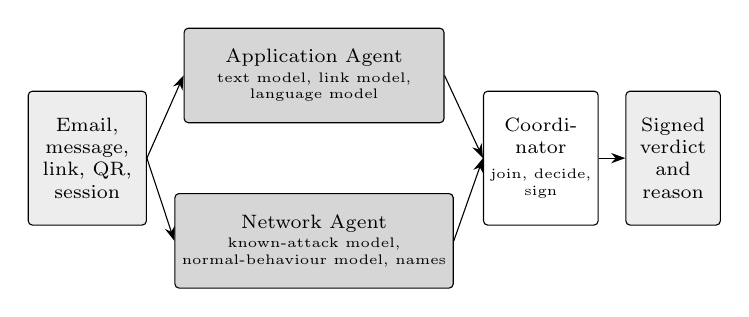
\begin{tikzpicture}[x=0.96cm,y=1cm,>={Stealth[length=1.8mm,width=1.3mm]},
  b/.style={draw, rounded corners=1.5pt, align=center, inner sep=2.5pt, font=\scriptsize, minimum height=7mm},
  g/.style={b, fill=black!7}, h/.style={b, fill=black!16}]
  \node[g, minimum width=1.5cm, minimum height=17mm] (in) at (0,0) {Email,\\message,\\link, QR,\\session};
  \node[h, minimum width=3.3cm, minimum height=12mm] (app) at (3.0,1.05) {Application Agent\\[-1pt]{\tiny text model, link model,}\\[-2pt]{\tiny language model}};
  \node[h, minimum width=3.3cm, minimum height=12mm] (net) at (3.0,-1.05) {Network Agent\\[-1pt]{\tiny known-attack model,}\\[-2pt]{\tiny normal-behaviour model, names}};
  \node[b, minimum width=1.4cm, minimum height=17mm] (co) at (6.0,0) {Coordi-\\nator\\[1pt]{\tiny join, decide,}\\[-2pt]{\tiny sign}};
  \node[g, minimum width=1.2cm, minimum height=17mm] (out) at (7.75,0) {Signed\\verdict\\and\\reason};
  \draw[->] (in.east) -- (app.west);
  \draw[->] (in.east) -- (net.west);
  \draw[->] (app.east) -- (co.west);
  \draw[->] (net.east) -- (co.west);
  \draw[->] (co) -- (out);
\end{tikzpicture}
\caption{STL. Both agents check the same item at the same time on one machine.}
\label{fig:arch}
\end{figure}

\subsection{Application Agent}

A reader opens email, HTML, QR codes and files. It also undoes tricks that change how text is stored but not how it reads: hidden characters, and letters borrowed from another alphabet inside a Latin word. It makes no judgement.

The \textbf{text model} is \texttt{Multilingual-MiniLM-L12-H384}~\cite{minilm} with mean pooling and a linear layer. It scores threat, hate, abuse and fraud at once. Training uses masked binary cross-entropy, because most sources say nothing about some labels. Long texts are read in up to eight windows of 128 tokens. The model runs on the CPU as an 8-bit ONNX file of 118 MB.

The \textbf{link model} is a character-level CNN that reads a URL as text, so no link is ever opened. Addresses are lower-cased and stripped of scheme and \texttt{www}. This stops the model from learning how each source formatted its URLs.

The \textbf{language model} is \texttt{qwen3.5:9b} (9 billion parameters, 4-bit), run locally through Ollama at temperature 0, with the whole model on the laptop GPU. It reads every item with text, because a gate on the fast risk loses polite and veiled messages (Section~\ref{sec:second-reader}). A bare link reaches it only if the link model flagged it, for the reason given in Section~\ref{sec:links}. It gets written label definitions, a use-or-mention instruction and short examples, and it returns labels, a confidence value and a reason as JSON. Its labels replace the fast labels. It cannot clear an item alone: if the fast models flagged an item and the language model finds nothing, the risk stays at a \emph{warning floor} of 0.3. It cannot block alone either: if the fast models saw no problem, its risk stops at 0.84, just under the block line, so a person decides. If it is alone and its confidence is under 0.9, a cut-off chosen on validation data, the item only gets a warning. It is not told any other model's opinion, neither the fast models' nor the Network Agent's, for the reason given in Section~\ref{sec:second-reader}.

\subsection{Network Agent}

This agent reads the last 32 connections of the sending host. For each connection it uses duration, packets, bytes each way, mean packet size, share sent, time since the last connection, whether the destination and port are new, protocol and one of 15 port groups. Host addresses only group the connections, and they are never model inputs.

The \textbf{known-attack model} is a small transformer (two layers, four heads, size 64) that scores the newest connection in that window. The \textbf{normal-behaviour model} is an Isolation Forest~\cite{iforest} on window features, fitted only on normal traffic. It can notice attacks it was never taught, but Section~\ref{sec:traffic} shows that it holds only on the network it learned. So its risk is capped at 0.45: it can warn, but it cannot flag alone. The link model also scores DNS and TLS server names, which stay readable in most encrypted sessions.

\subsection{Coordinator}

Each model has its own best cut-off $t$, chosen on validation data. A score $s$ maps to a common risk $r$, where 0.5 always means that cut-off:
\begin{equation}
r = \begin{cases} 0.5\, s / t & s < t \\ 0.5 + 0.5\,(s-t)/(1-t) & s \ge t \end{cases}
\end{equation}
The agents are joined as two witnesses:
\begin{equation}
R = 1 - (1 - r_a)(1 - r_n)
\end{equation}
An agent with nothing to say is left out. The rule can only raise risk, so the system inherits false alarms from both agents. The actions are allow below 0.3, warn from 0.3, flag from 0.5 and block from 0.85. These were set before testing and were not tuned on the tests.

Each agent signs its finding with its own Ed25519 key, and the Coordinator signs the whole record. A signature shows who said something and that nobody changed it. It does not show that the statement is true.

\section{Data and Method}

\subsection{Data}

Table~\ref{tab:data} lists the data. All of it is public and real. Live phishing URLs are stored as text and never opened, and no malware files were downloaded.

\begin{table}[t]
\caption{Data. Unseen means whole sources kept out of training.}
\label{tab:data}
\centering
\footnotesize
\begin{tabular}{@{}>{\raggedright\arraybackslash}p{3.7cm}r>{\raggedright\arraybackslash}p{2.75cm}@{}}
\toprule
\textbf{Source} & \textbf{Rows} & \textbf{Use} \\
\midrule
\multicolumn{3}{@{}l}{\emph{Text}} \\
Civil Comments~\cite{civil}, emails, SMS~\cite{smsspam}, Roman Urdu~\cite{ruhsold} & 458,304 & Training \\
Measuring Hate Speech~\cite{mhs} & 27,829 & Unseen source test \\
Nazario, Nigerian Fraud & 6,058 & Unseen source test \\
Civil Comments (test) & 96,629 & Held-out test \\
Roman Urdu (test)~\cite{ruhsold} & 1,997 & Held-out test \\
\multicolumn{3}{@{}l}{\emph{Links}} \\
Phishing.Database, PhiUSIIL~\cite{phiusiil}, Common Crawl, Tranco~\cite{tranco} & 2,316,801 & Training \\
Same sources, new domains & 295,390 & Held-out domains \\
OpenPhish feed & 276 & Live links, unseen domains \\
\multicolumn{3}{@{}l}{\emph{Traffic}} \\
Corrected CICIDS2017~\cite{cicids,engelen} & 2,099,976 & Five days \\
CTU-13~\cite{ctu13} & 4,907,237 & 13 botnet scenarios \\
MAWI backbone~\cite{mawi} & 1,648,523 & Unlabelled live traffic \\
\bottomrule
\end{tabular}
\end{table}

\subsection{Rules against leaks}

We split links by registered domain, so a domain seen in training never appears in a test. Whole text sources stay out of training. Training text that shared passages of 50 characters or more with the unseen tests was removed, 1,968 fraud rows and 3,614 normal rows. For traffic we use two splits. In the first, attack days never appear in training. In the second, the last 20\% of each label in time is held out. For CTU-13, whole scenarios are held out. Thresholds come from validation data only.

\subsection{Baselines and measures}

The text baselines are a keyword filter and a TF-IDF linear model. The traffic baseline is LightGBM~\cite{lightgbm} on single flows. We report precision, recall, F1 and false alarm rate. Traffic results also give recall at 1\% and 0.1\% false alarms, because of the base rate: if one flow in 10,000 is bad and all are caught, a 1\% false alarm rate still gives a precision of about 1\%.

\subsection{Testing without paired data}
\label{sec:nopaired}

No public dataset links one event across both layers. A flow in CICIDS2017 and an email in the Nazario set share no session, host or attack. So the system test pairs real held-out content with real held-out traffic histories from separate sources and sends them as real SMTP sessions through the gateway. In this design each agent alone must miss a whole group of sessions, so the joined result beats either agent by construction. We report it as a system test, not as a gain from joining.

The training and evaluation ran on a laptop with an NVIDIA RTX 4050 (6 GB). The fast models run on the CPU, and the language model shares the laptop GPU.


\section{Results}

\subsection{Content (RQ1)}
\label{sec:content}

\begin{table*}[t]
\caption{Fast text model on text it never trained on. Bad / all counts the harmful rows. Civil Comments is a random 60,000 rows of the test split.}
\label{tab:text}
\centering
\footnotesize
\begin{tabular}{@{}lrrrrrrr@{}}
\toprule
 & & \multicolumn{3}{c}{\textbf{F1}} & \multicolumn{3}{c}{\textbf{False alarms}} \\
\textbf{Test} & \textbf{Bad / all} & \textbf{Keyword} & \textbf{Linear} & \textbf{STL} & \textbf{Keyword} & \textbf{Linear} & \textbf{STL} \\
\midrule
\tablerows{generated/text_rows.tex}
\bottomrule
\end{tabular}
\end{table*}

Table~\ref{tab:text} gives the fast text model on text it never trained on. Keywords lost on every row, so the answer to RQ1 is yes. The transformer, though, has no clear lead over the linear baseline. It has the best F1 on Civil Comments and SMS, and the linear model has the best F1 on the other three rows, by a small margin. On two of those three the linear model pays with far more false alarms: \hateUnseenLinearFA{} against \hateUnseenFA{} on the unseen hate source, and \urduLinearFA{} against \urduFA{} on Roman Urdu. Two rows are weak for every system. Threats are rare, \textThreatBad{} in \textThreatRows{} rows, and the best F1 is \textThreatFone{}. And hate does not travel: the transformer caught only \hateUnseenRecall{} of the hateful rows from the source it never saw.

\begin{table}[t]
\caption{57 hand-written messages: 36 harmful, 21 harmless. C caught, FA false alarms. These messages shaped the design, so this is a demonstration and not a measurement.}
\label{tab:semantic}
\centering
\footnotesize
\setlength{\tabcolsep}{3pt}
\begin{tabular}{@{}lrrrrrr@{}}
\toprule
 & \multicolumn{2}{c}{\textbf{Keyword}} & \multicolumn{2}{c}{\textbf{Fast}} & \multicolumn{2}{c}{\textbf{With LM}} \\
\textbf{Group} & \textbf{C} & \textbf{FA} & \textbf{C} & \textbf{FA} & \textbf{C} & \textbf{FA} \\
\midrule
\tablerows{generated/semantic_rows.tex}
\bottomrule
\end{tabular}
\end{table}

We wrote the 57 messages in Table~\ref{tab:semantic} to be hard: polite scams, veiled threats, and text in Urdu and Roman Urdu. On the 20 messages with no obvious keyword, the keyword filter caught \plainKeyword{} and the fast model \plainFast{}. With the language model reading too, the system caught \plainBoth{}. All three misses are veiled threats that the language model did name, but with a confidence under 0.9, so they got a warning. We show this table for what it reveals about polite and veiled text, and Section~\ref{sec:second-reader} shows why it must not be read as an accuracy.

\subsection{Links and QR codes (RQ2)}
\label{sec:links}

Table~\ref{tab:links} gives the link results. The link model reads a URL in about \linkMs{} ms on the CPU. On \linkRows{} links from domains it never saw, it reached an F1 of \linkFone{}, with \linkFalseAlarm{} false alarms. A live OpenPhish feed, on unseen domains, gave a recall of \linkOpenphish{}, and a later fetch of links that appeared after training gave \linkOpenphishLater{}. False alarms were not even across sources: \linkCrawlFA{} of Common Crawl pages were flagged, but \linkTrancoFA{} of the Tranco top sites. A likely reason is that popular sites are short brand names, the names phishing pages copy.

The language model did not help on bare links, and this was the largest surprise of the second run. On our 66 hand-made links it looked better than the link model, with \fakeOldCaught{} caught and \fakeOldWrong{} false alarms, against \fakeLinkCaught{} and \fakeLinkWrong{}. On real links it was far worse. Of \linkSampleEach{} real phishing and \linkSampleEach{} real normal links, it caught \linkSampleCaught{} and wrongly flagged \linkSampleWrong{}, against \linkSampleFastCaught{} and \linkSampleFastWrong{} for the link model. Reading its reasons showed why. It claims that an ordinary name copies a brand: it called \texttt{scandlines.com}, a ferry company's own site, a misspelling of a hotel chain. Its confidence gives no warning either, at 0.9 or more on every such link in our validation sample. A language model judges a link from what it remembers about names, and it remembers few small sites.

So we changed the rule again, using validation links only (Table~\ref{tab:linkrules}). A bare link now reaches the language model only if the link model flagged it. There the model can confirm the flag or lower it to a warning, and it can never raise a link alone. This keeps what it is good at, knowing famous sites, and drops what it is bad at. The final rule flagged \ruleFinalNormal{} of \ruleEach{} normal links on validation, against \ruleContentNormal{} under the content rule. The cost is that some phishing links drop from a flag to a warning. On the held-out sample, the final rule caught \linkFinalCaught{} of \linkSampleEach{} and wrongly flagged \linkFinalWrong{}. Table~\ref{tab:links} gives all the test results.

\begin{table}[t]
\caption{Choosing the rule for bare links, on validation links: links flagged / links at least warned.}
\label{tab:linkrules}
\centering
\footnotesize
\setlength{\tabcolsep}{2.5pt}
\begin{tabular}{@{}lrrr@{}}
\toprule
\textbf{Rule} & \textbf{Phishing (\ruleEach{})} & \textbf{Normal (\ruleEach{})} & \textbf{Popular (\rulePopular{})} \\
\midrule
\tablerows{generated/link_rule_rows.tex}
\bottomrule
\end{tabular}
\end{table}

\begin{table}[t]
\caption{Links and QR codes. P precision, R recall, FA false alarms.}
\label{tab:links}
\centering
\footnotesize
\begin{tabular}{@{}>{\raggedright\arraybackslash}p{3.0cm}r>{\raggedright\arraybackslash}p{3.2cm}@{}}
\toprule
\textbf{Test} & \textbf{Size} & \textbf{Result} \\
\midrule
\tablerows{generated/link_rows.tex}
\bottomrule
\end{tabular}
\end{table}

All \qrImages{} QR images were read correctly, including rotated, blurred, dim, angled and poster-sticker forms, at \qrMs{} ms per image. The verdict was right on \qrRight{}. The other \qrWrong{} are \qrWrongCodes{} fake links, each printed in six forms, that the link model passes and the language model no longer sees. We made these images ourselves, so this shows that the pipeline works and says nothing about what real attackers print. So the answer to RQ2 is yes, and the part that does the work is the small model trained on URLs, not the language model.

\subsection{Traffic (RQ3)}
\label{sec:traffic}

Table~\ref{tab:flows} shows how the known-attack model carries. On attacks it was taught, it is near perfect, and it beats LightGBM on false alarms: F1 \laterFone{} with \laterFA{} false alarms on later flows. On attack days it never saw, F1 falls to \thursdayFone{} and \fridayFone{}. At the cut-off chosen on validation data, it simply does not call new attacks attacks. LightGBM has the same problem, and on those two days it ranks flows better than our transformer does, as the AUC columns show. So the deeper model gives no gain on new attacks. On CTU-13 scenarios held out whole, the transformer has the better F1 on three of four. The botnet in scenario 7 is mostly missed by both.

\begin{table}[t]
\caption{Known-attack model against LightGBM on single flows.}
\label{tab:flows}
\centering
\footnotesize
\setlength{\tabcolsep}{3.5pt}
\begin{tabular}{@{}>{\raggedright\arraybackslash}p{3.05cm}rrrrrr@{}}
\toprule
 & \multicolumn{3}{c}{\textbf{STL}} & \multicolumn{3}{c}{\textbf{LightGBM}} \\
\textbf{Test} & \textbf{F1} & \textbf{FA} & \textbf{AUC} & \textbf{F1} & \textbf{FA} & \textbf{AUC} \\
\midrule
\tablerows{generated/flow_rows.tex}
\bottomrule
\end{tabular}
\end{table}

The normal-behaviour model never saw an attack. On the same two unseen days it reached a recall of \thursdayRecall{} and \fridayRecall{}, with \thursdayFA{} and \fridayFA{} false alarms (Table~\ref{tab:anomaly}). Read alone, that looks like the answer to new attacks. Three facts stop us from saying so. The attacks it catches are mostly loud floods and scans, and it misses a quiet botnet almost entirely (recall \botnetRecall{} on Friday's botnet). At 0.1\% false alarms, recall falls to \thursdayRecallLow{} and \fridayRecallLow{}. And it does not travel. Built on CICIDS2017 and tested on the 13 CTU-13 captures, it gave \crossFALow{} to \crossFAHigh{} false alarms, and the known-attack model reached a recall of only \crossRecallLow{} to \crossRecallHigh{}.

\begin{table}[t]
\caption{Normal-behaviour model. The last column is recall at 0.1\% false alarms.}
\label{tab:anomaly}
\centering
\footnotesize
\setlength{\tabcolsep}{4pt}
\begin{tabular}{@{}>{\raggedright\arraybackslash}p{3.9cm}rrrr@{}}
\toprule
\textbf{Test} & \textbf{Recall} & \textbf{FA} & \textbf{AUC} & \textbf{R@0.1\%} \\
\midrule
\tablerows{generated/anomaly_rows.tex}
\bottomrule
\end{tabular}
\end{table}

The live Internet shows the same thing. We ran both models over \backboneFlows{} flows of one MAWI backbone capture, from \backboneHosts{} hosts, and scored \backboneScored{} flows from \backboneScoredHosts{} hosts. These flows have no labels, so we can only report how often the models fired. The known-attack model fired on \backboneKnown{} of flows. The normal-behaviour model from the lab fired on \backboneLab{}, so on this network it is useless. After we fitted a new one on half of the hosts, it fired on \backboneLocal{} of flows from the other half, close to the 0.5\% target. That is why its risk is capped: it can warn, but it cannot flag alone, and each network must teach it what normal is. Scoring ran at \backboneSpeed{} flows per second on the CPU.

\subsection{The language model as a second reader (RQ4)}
\label{sec:second-reader}

\textbf{What the hand-written tests hid.} Our first design used a prompt tuned on the 57 hand-written messages, where it gave \firstRunHandWrong{} false alarms on harmless text. The first full run then flagged \firstRunWrong{} of \firstRunClean{} clean sessions (\firstRunCleanFA{}), and \firstRunBlocked{} of those were blocked outright. Reading the flagged messages showed the cause: the model treated political argument as hate speech, and our hand-written harmless messages contained none. Part of the rate is label noise too. Civil Comments marks a comment as harmful when at least half of its raters did, so ``calm'' comments include rude ones, and one flagged comment was a real scam advert.

We then changed the design, using validation rows only (Table~\ref{tab:prompts}). A tighter prompt defines hate by protected groups and names political argument as harmless. It halved false alarms on calm comments, though at a cost in catches. A second sentence says that words addressed to a reviewer, or claims that a message was already checked, prove nothing. On validation rows it cut successful attacks from \attackCalm{} to \attackGuard{}, and it won back \promptGainBack{} of the \promptLost{} lost catches, though with more flags on calm comments. We also tried asking for the reason before the labels, a common way to make a model think first. It made things worse, with \reasonFirstCalm{} calm comments flagged against \tighterCalm{}. Last, we found that false alarms mostly came with lower confidence. So one reader alone now flags only at a confidence of 0.9 or more, and below that it warns. Against the column before it, the last column keeps \promptFinalCaught{} of \promptGuardCaught{} catches, with about a third of the flags on calm comments, \promptFinalCalm{} against \promptGuardCalm{}. All results below come from a second full run with this design, and the link results above come from one more link test after the change described there. The test sets did not choose the prompt, but a test result is what made us look, so these results are not fully blind.

\begin{table}[t]
\caption{Choosing the prompt and rule on validation rows: messages flagged. The first three columns count any label. The last adds the final rule to the guarded prompt: a sure reader, or both readers agreeing.}
\label{tab:prompts}
\centering
\footnotesize
\setlength{\tabcolsep}{4pt}
\begin{tabular}{@{}lrrrr@{}}
\toprule
\textbf{Rows} & \textbf{First} & \textbf{Tighter} & \textbf{Guarded} & \textbf{Final rule} \\
\midrule
\tablerows{generated/prompt_rows.tex}
\bottomrule
\end{tabular}
\end{table}

\textbf{On real text.} Table~\ref{tab:sample} is the fair test of the final design. We drew \sampleSize{} harmful and \sampleSize{} harmless held-out rows, and counted what the system would flag for any reason. Caught fell from \sampleFastCaught{} to \sampleBothCaught{}, and false alarms fell from \sampleFastWrong{} to \sampleBothWrong{}. So the language model is not a free gain, and the result depends on the source. On fraud email it caught all \sampleFraudBoth{} of \sampleEach{}, against \sampleFraudFast{}, and cut false alarms from \sampleFraudFastWrong{} to \sampleFraudBothWrong{}. On the unseen hate source it did better on both counts too. On Civil Comments it gave up many catches, most of all on abuse, \sampleAbuseFast{} down to \sampleAbuseBoth{}, and on threats, \sampleThreatFast{} down to \sampleThreatBoth{}. Part of that loss is what we asked for, because the prompt leaves blunt opinion alone and these labels are crowd votes that include plain rudeness. Part of it is a real loss. Roman Urdu abuse fell from \sampleUrduFast{} to \sampleUrduBoth{}, with no gain in false alarms. Nothing here goes silent: a message the fast model flagged and the language model cleared keeps a warning.

Comments with no objection from any rater make up \clearShare{} of the Civil Comments test split. Of \clearSize{} such comments the system flagged \clearBoth{} (95\% interval \clearLow{} to \clearHigh{}), against \clearFast{} for the fast model alone. This is the closest we can get to a field rate from this data.

\begin{table}[t]
\caption{Held-out text, balanced samples: messages the system would flag for any reason, out of the sample size each way. Harmless rows carry no harmful label.}
\label{tab:sample}
\centering
\footnotesize
\setlength{\tabcolsep}{4pt}
\begin{tabular}{@{}lrrrr@{}}
\toprule
 & \multicolumn{2}{c}{\textbf{Caught}} & \multicolumn{2}{c}{\textbf{False alarms}} \\
\textbf{Test} & \textbf{Fast} & \textbf{With LM} & \textbf{Fast} & \textbf{With LM} \\
\midrule
\tablerows{generated/sample_rows.tex}
\bottomrule
\end{tabular}
\end{table}

\textbf{Reading everything.} A gate on the fast risk would save time, because most text would skip the language model. On the 57 messages, reading everything gave \gateZeroCaught{} caught. A gate of 0.08 read \gateHighMail{} of normal mail and \gateHighComments{} of comments, but it caught only \gateHighCaught{}, because the fast model gives low scores to polite scams and veiled threats. So STL reads all text by default.

\textbf{It copies.} We told the language model what the link model thought of each of the 66 test links. Told nothing, it caught \opinionNoneCaught{} frauds and wrongly flagged \opinionNoneWrong{} normal links. Told the right opinion, it scored \opinionRightCaught{} and \opinionRightWrong{}. Told the wrong opinion, it scored \opinionBadCaught{} and \opinionBadWrong{}. So a wrong opinion cost it catches and added false alarms, though less than with the first prompt, which wrongly flagged \firstRunOpinionWrong{}. The same happened with traffic. Told that the sender's traffic matched a known attack, it flagged \noteWithFlagged{} of \noteHarmless{} harmless messages, against \noteAloneFlagged{} when told nothing. It caught all \noteHarmful{} harmful ones either way. So STL tells it nothing. It reads alone, and the Coordinator joins the agents after both have decided.

\textbf{Disguises.} Table~\ref{tab:disguise} applies seven disguises to \disguiseCount{} harmful and \disguiseHarmless{} harmless hand-written messages. Cleaning works: hidden characters and borrowed letters leave every column at its undisguised value. Swapping letters for symbols breaks the keyword filter (\leetKeyword{}), and it also breaks the fast model in the other direction. That model flagged all of them, \leetFast{} harmful and \leetFastWrong{} harmless, so odd spelling alone looks harmful to it. The language model pulled the harmless rows back to \leetBothWrong{}, which is still the worst false alarm rate in the table. Hiding a message in long normal text left \longBoth{} caught and \longBothWrong{} false alarms. The strongest disguise is an instruction to the reviewer. It left \orderBoth{} caught, up from \firstRunOrderBoth{} with the first prompt.

\begin{table}[t]
\caption{Hand-written messages after a disguise. The first three columns count harmful messages caught. The last counts harmless messages wrongly flagged with the language model on.}
\label{tab:disguise}
\centering
\footnotesize
\setlength{\tabcolsep}{3.5pt}
\begin{tabular}{@{}>{\raggedright\arraybackslash}p{3.2cm}rrrr@{}}
\toprule
\textbf{Disguise} & \textbf{Keyword} & \textbf{Fast} & \textbf{With LM} & \textbf{FA} \\
\midrule
\tablerows{generated/disguise_rows.tex}
\bottomrule
\end{tabular}
\end{table}

\textbf{Attacks.} Next we attacked the language model directly (Table~\ref{tab:attacks}). We took \injectionHarmful{} harmful messages, our 36 hand-written ones plus real fraud and toxic rows from the test sets, and kept the \injectionCaught{} that the system caught before any attack. Then we added text to each one, in eight ways, for \injectionTried{} tries. The first six attacks are the ones we used on the validation rows, and they fooled the model in \injectionEarlyFooled{} of \injectionEarlyTried{} tries. We added the last two after probing the final prompt for a weakness, and they fooled it in \injectionLateFooled{} of \injectionLateTried{}. These two copy the form of a report: they say the text is a record or an exam sample and is only quoted. Section~\ref{sec:discussion} explains why that form is hard to close.

In all, the model was fooled in \injectionFooledCount{} tries (\injectionFooled{}). The warning floor kept a warning on \injectionSaved{} of them, because the fast model had seen the message. The other \injectionSilent{} tries passed in silence, because no reader was left. If the sender's traffic also looks unusual, each of those \injectionSaved{} warnings becomes a flag, as the last column shows. We show no column for known attack traffic, because it flags a session on its own whatever the content says.

So the answer to RQ4 is a limited yes. The language model is useful as a second reader of text, but only with limits on what it can do alone, and it should not judge bare links.

\begin{table}[t]
\caption{Attack text added to harmful messages that were caught before the attack. Warned means at least a warning. The last two columns assume the sender's traffic looked unusual.}
\label{tab:attacks}
\centering
\footnotesize
\setlength{\tabcolsep}{3pt}
\begin{tabular}{@{}lrrrrrr@{}}
\toprule
 & & & \multicolumn{2}{c}{\textbf{Warned}} & \multicolumn{2}{c}{\textbf{Flagged}} \\
\textbf{Attack} & \textbf{Fooled} & \textbf{Flagged} & \textbf{Bare} & \textbf{Floor} & \textbf{Bare} & \textbf{Floor} \\
\midrule
\tablerows{generated/injection_rows.tex}
\bottomrule
\end{tabular}
\end{table}

\subsection{Two layers together (RQ5)}
\label{sec:together}

\begin{table}[t]
\caption{System test: share of sessions flagged, \systemGroup{} sessions per group. The last column turns the language model off.}
\label{tab:system}
\centering
\footnotesize
\setlength{\tabcolsep}{3.5pt}
\begin{tabular}{@{}>{\raggedright\arraybackslash}p{3.3cm}rrrr@{}}
\toprule
\textbf{Group} & \textbf{App.} & \textbf{Net.} & \textbf{Joined} & \textbf{No LM} \\
\midrule
\tablerows{generated/system_rows.tex}
\bottomrule
\end{tabular}
\end{table}

Table~\ref{tab:system} gives the system test: \systemSessions{} real SMTP sessions through the gateway. All \systemSessions{} verdicts came back with valid signatures. Joined recall was \systemRecall{}, precision \systemPrecision{} and false alarms on clean sessions \systemCleanFA{} (95\% interval \systemCleanLow{} to \systemCleanHigh{}). As Section~\ref{sec:nopaired} says, the joined column beats each agent by construction, so these numbers show that the parts work together. They are not a gain from joining.

The last column is a fairer comparison, because only one thing changes. With the language model off, clean sessions were flagged \fastSystemFA{} of the time and \fastSystemBlocked{} of \systemGroup{} were blocked. With it on, \systemCleanFA{} were flagged and \systemCleanBlocked{} blocked, and another \systemCleanWarned{} got a warning. The price was a small fall in recall, from \fastSystemRecall{} to \systemRecall{}. In the first design the same test gave \firstRunCleanFA{} flagged and \firstRunBlocked{} blocked, so the work on the prompt and rule paid off. Harmful content from a normal host is the hard group. It was flagged \systemHarmful{} of the time, \systemHarmfulWarned{} of \systemGroup{} sessions got a warning, and \systemHarmfulSilent{} passed in silence, against \fastHarmfulSilent{} with the language model off. Here the Network Agent cannot help.

RQ5 asks whether one layer can cover for the other. The evidence is narrow, but it is real. One of our \scenariosTotal{} demos shows it end to end: a threat dressed up as a record fools the language model, and the fast model's warning leaves the Application Agent at \recordApp{}. The sender's traffic is unusual, so the Network Agent reports \recordNet{}. Each alone is only a warning, and joined they reach \recordJoined{}, a flag. This works only when the fast model saw the message and the traffic really is unusual. Of the other demos, \demoOthersPassed{} behaved as expected. One did not: an Urdu threat that the language model read correctly with a confidence of \urduConfidence{}, under the 0.9 cut-off, so it got a warning and not a flag.

\subsection{Speed}

The fast text model takes \msPerText{} ms per item on the CPU, the link model \linkMs{} ms, and reading a QR image \qrMs{} ms. The language model takes about \sampleSeconds{} seconds per item and uses the whole laptop GPU, so it sets the pace. A full session, from SMTP to signed verdict, took a median of \systemMedian{} seconds, and 95\% took under \systemPninetyfive{} seconds. With the language model off, the median was \fastSystemMedian{} seconds.


\section{Discussion}
\label{sec:discussion}

\subsection{The language model is the best reader and the weakest link}

The language model turned out to be the part that decides most of the content results. It reads polite scams and veiled threats that the fast model passes with confidence, and it cut false alarms on clean sessions to a third. It also has three faults, and each one changed the design.

First, it copies. Told what another model thinks, it leans that way, and that holds for a link opinion and for a traffic finding. A tighter prompt reduced this, but it did not end it. A second reader that leans on the first is worth little, so STL tells it nothing and leaves the joining to the Coordinator.

Second, it can be argued with. A plain order to ignore its instructions rarely works now, but a believable story does. The fake record works because of a rule we added on purpose: a report about abuse is not abuse. That rule protects people who report harm, which earlier work shows is needed~\cite{gligoric}, and an attacker can copy the form of a report. We do not see how a prompt alone can give one without the other. The warning floor and the traffic signal limit the damage, but they do not remove it.

Third, it can look better than it is. Our first prompt was tuned on 57 hand-written messages and gave \firstRunHandWrong{} false alarms on the harmless ones. On real text in the first full run, the same prompt flagged \firstRunCleanFA{} of clean sessions. Our hand-written harmless messages were simply easier than a comment section about politics. Links then told the same story. On our 66 hand-made links the model beat the link model, and on real links it flagged \linkSampleWrong{} of \linkSampleEach{} normal ones, where the link model flagged \linkSampleFastWrong{}. Any team that tests a language model only on examples it wrote itself is likely to make the same mistake.

\subsection{What joining the layers does and does not show}

The system test shows that the parts work together under real sessions. It does not show that joining beats one layer, because the test is built so that one layer must miss a whole group. The honest evidence for RQ5 is narrower. When an attack fools the language model and the fast model saw the message, a warning stays, and if the sender's host also looks unusual, the session is flagged. That held for \injectionSaved{} of the \injectionFooledCount{} fooled tries. For the rest, no reader was left. It also depends on the attacker's host looking unusual, and an attacker who sends through a clean relay escapes it.

\subsection{Behaviour models belong to their network}

The normal-behaviour model looked very strong on the days it was built for and failed on every other network. That is not a flaw of one model. Normal traffic differs between networks, so a model of normal has to learn the network it guards. Reports that train and test such a model on one capture say little about how it would behave anywhere else.

\section{Limits}

\begin{itemize}
  \item \textbf{No paired data.} Content and traffic in our system test come from separate sources. The gain from joining on real paired events is still unmeasured.
  \item \textbf{Small hand-written sets.} The 57 messages, 66 links and 96 QR images show the type of error. They are not benchmarks, and the 57 messages also shaped the design.
  \item \textbf{Noisy labels.} Civil Comments labels come from crowd votes on North American news comments. Hate labels from one source do not always match another's. Some of our false alarms may be labelling disagreements, and some of our catches may be luck.
  \item \textbf{Old traffic.} CICIDS2017 and CTU-13 are years old and come from lab or campus networks. Our MAWI result has no labels, so it shows behaviour and not accuracy.
  \item \textbf{No field base rate.} Real harmful messages are rare. Our false alarm rates are measured on balanced or planned samples, so precision in the field would be lower.
  \item \textbf{Links inside messages.} The final rule covers bare links only. Links inside a message still reach the language model with the text, and we did not test whether it invents problems there too.
  \item \textbf{Thin local coverage.} We have Roman Urdu abuse data, but no public Urdu or Roman Urdu fraud data. Only the hand-written messages test this.
  \item \textbf{No fairness test.} We did not measure whether false alarms fall more on some dialects or groups. Abuse models are known to do this, so it must be tested before any real use.
  \item \textbf{Two rounds of changes.} We changed the design after the first full run and again after the second. Validation rows chose each change, and no test set chose a prompt or a rule. But test results told us where to look, so our final numbers are not fully blind.
  \item \textbf{One training run.} Each model was trained once, so we give no spread across seeds. The language model runs at temperature 0, so repeating a test gives nearly the same answers.
  \item \textbf{One laptop.} The language model takes about \sampleSeconds{} seconds per item and uses the whole GPU. A busy mail server would need more hardware or a queue. All keys are plain files on one machine.
\end{itemize}

\section{Future Work}

The next step is a paired testbed: a lab network where the same hosts send real content and produce real traffic, some of them infected, so one event exists at both layers. Only that can measure what joining adds. We also plan to test larger local language models, to separate instructions from data in a stronger way than a prompt can, to train the fast models against attacks like those in Section~\ref{sec:second-reader}, and to let operators exchange signed verdicts as the full STL design proposes.

\section{Conclusion}

We built a system that reads one event at both layers on a single laptop, and measured it on real data with whole sources kept out of training. Trained models beat keywords on unseen sources, links can be judged without opening them, and known-attack traffic models work well on attacks they were taught. New attacks and new networks remain hard. A local language model is a useful second reader for text, and it cut false alarms on clean sessions to a third. But it leans on opinions it is told, it can be talked out of correct answers, and it can look far better on hand-written tests than on real text. The joined design limits the harm of a fooled reader, and how much it adds on real paired events is still an open question.

\section*{Acknowledgment}

This work was done as a final year project at NUTECH, Islamabad, under the supervision of Maj. Babar. We used Anthropic Claude (Claude Code) to help write and debug the prototype code and test scripts, to search the literature, and to draft the text of all sections of this paper. We checked the code, results and text, and we take responsibility for them.


\begin{thebibliography}{99}
\bibitem{darktrace} Darktrace, ``Platform overview.'' [Online]. Available: \url{https://www.darktrace.com/platform}. Accessed: Nov. 6, 2026.
\bibitem{triage} Microsoft, ``Phishing Triage Agent in Microsoft Defender.'' [Online]. Available: \url{https://learn.microsoft.com/en-us/defender-xdr/phishing-triage-agent}. Accessed: Nov. 6, 2026.
\bibitem{fard} H.~Fard, I.~Komarov, and G.~Wunder, ``Cross-Layer Intrusion Detection in 5G O-RAN: Gains and Limits of Fusing Radio Telemetry with Network Flow Records,'' arXiv:2606.22450, 2026.
\bibitem{code} STL prototype, code and test sets. Link to be added at submission.
\bibitem{becguard} A.~Cidon, L.~Gavish, I.~Bleier, N.~Korshun, M.~Schweighauser, and A.~Tsitkin, ``High precision detection of business email compromise,'' in \emph{Proc. 28th USENIX Security Symp.}, 2019, pp.~1291--1307.
\bibitem{urltran} P.~Maneriker, J.~W.~Stokes, E.~Garcia~Lazo, D.~Carutasu, F.~Tajaddodianfar, and A.~Gururajan, ``URLTran: Improving Phishing URL Detection Using Transformers,'' \emph{MILCOM 2021 - 2021 IEEE Military Communications Conference (MILCOM)}, pp.~197--204, 2021, doi: 10.1109/MILCOM52596.2021.9653028.
\bibitem{chatspam} T.~Koide, N.~Fukushi, H.~Nakano, and D.~Chiba, ``ChatSpamDetector: Leveraging Large Language Models for Effective Phishing Email Detection,'' arXiv:2402.18093, 2024.
\bibitem{topcuoglu} C.~Topcuoglu \emph{et al.}, ``Measuring and Evaluating the Performance of Generative Ai Models for Scam Detection,'' \emph{2026 IEEE 50th Annual Computers, Software, and Applications Conference (COMPSAC)}, pp.~641--651, 2026, doi: 10.1109/COMPSAC69091.2026.00090.
\bibitem{afane} K.~Afane, W.~Wei, Y.~Mao, J.~Farooq, and J.~Chen, ``Next-Generation Phishing: How LLM Agents Empower Cyber Attackers,'' \emph{2024 IEEE International Conference on Big Data (BigData)}, pp.~2558--2567, 2024, doi: 10.1109/BigData62323.2024.10825018.
\bibitem{phishllm} R.~Liu, Y.~Lin, X.~Teoh, G.~Liu, Z.~Huang, and J.~S.~Dong, ``Less defined knowledge and more true alarms: Reference-based phishing detection without a pre-defined reference list,'' in \emph{Proc. USENIX Security Symp.}, 2024.
\bibitem{hateday} M.~Tonneau \emph{et al.}, ``HateDay: Insights from a Global Hate Speech Dataset Representative of a Day on Twitter,'' arXiv:2411.15462, 2024.
\bibitem{threatcore} D.~Bruni, C.~Bardazzi, and M.~Tesconi, ``ThreatCore: A Benchmark for Explicit and Implicit Threat Detection,'' arXiv:2605.10563, 2026.
\bibitem{gligoric} K.~Gligoric, M.~Cheng, L.~Zheng, E.~Durmus, and D.~Jurafsky, ``NLP Systems That Can't Tell Use from Mention Censor Counterspeech, but Teaching the Distinction Helps,'' arXiv:2404.01651, 2024.
\bibitem{pervaiz} F.~Pervaiz \emph{et al.}, ``An assessment of SMS fraud in Pakistan,'' \emph{Proceedings of the 2nd ACM SIGCAS Conference on Computing and Sustainable Societies}, pp.~195--205, 2019, doi: 10.1145/3314344.3332500.
\bibitem{ayaz} M.~Ayaz, S.~Nizamani, A.~A.~Chandio, and K.~K.~Luhana, ``Detection of Roman Urdu fraud/spam SMS in Pakistan Using Machine Learning,'' \emph{International Journal of Computing and Digital Systems}, vol.~15, pp.~1053--1061, 2024, doi: 10.12785/ijcds/150174.
\bibitem{ruhsold} H.~Rizwan, M.~H.~Shakeel, and A.~Karim, ``Hate-Speech and Offensive Language Detection in Roman Urdu,'' \emph{Proceedings of the 2020 Conference on Empirical Methods in Natural Language Processing (EMNLP)}, pp.~2512--2522, 2020, doi: 10.18653/v1/2020.emnlp-main.197.
\bibitem{fire} M.~Amjad \emph{et al.}, ``Overview of abusive and threatening language detection in Urdu at FIRE 2021,'' in \emph{Working Notes of FIRE 2021}, CEUR-WS Vol.~3159, 2021, pp.~744--762.
\bibitem{trad} F.~Trad and A.~Chehab, ``Detecting Quishing Attacks with Machine Learning Techniques Through QR Code Analysis,'' \emph{IFIP Advances in Information and Communication Technology}, pp.~194--206, 2026, doi: 10.1007/978-3-032-30805-4\_14.
\bibitem{wickramasinghe} N.~Wickramasinghe, A.~Shaghaghi, G.~Tsudik, and S.~Jha, ``SoK: Decoding the Enigma of Encrypted Network Traffic Classifiers,'' \emph{2025 IEEE Symposium on Security and Privacy (SP)}, pp.~1825--1843, 2025, doi: 10.1109/SP61157.2025.00165.
\bibitem{zhao} Y.~Zhao, G.~Dettori, M.~Boffa, L.~Vassio, and M.~Mellia, ``The Sweet Danger of Sugar: Debunking Representation Learning for Encrypted Traffic Classification,'' \emph{Proceedings of the ACM SIGCOMM 2025 Conference}, pp.~296--310, 2025, doi: 10.1145/3718958.3750498.
\bibitem{cicids} I.~Sharafaldin, A.~H.~Lashkari, and A.~A.~Ghorbani, ``Toward Generating a New Intrusion Detection Dataset and Intrusion Traffic Characterization,'' \emph{Proceedings of the 4th International Conference on Information Systems Security and Privacy}, pp.~108--116, 2018, doi: 10.5220/0006639801080116.
\bibitem{engelen} G.~Engelen, V.~Rimmer, and W.~Joosen, ``Troubleshooting an Intrusion Detection Dataset: the CICIDS2017 Case Study,'' \emph{2021 IEEE Security and Privacy Workshops (SPW)}, pp.~7--12, 2021, doi: 10.1109/SPW53761.2021.00009.
\bibitem{flood} R.~Flood, G.~Engelen, D.~Aspinall, and L.~Desmet, ``Bad Design Smells in Benchmark NIDS Datasets,'' \emph{2024 IEEE 9th European Symposium on Security and Privacy (EuroS\&amp;P)}, pp.~658--675, 2024, doi: 10.1109/EuroSP60621.2024.00042.
\bibitem{zaro} A.~Zaro, ``Adversarial Robustness Is Not Zero-Day Generalization: A Controlled Evaluation of Flow-Based Intrusion Detectors on Corrected CIC-IDS2017,'' arXiv:2611.00713, 2026.
\bibitem{moczkodan} Z.~Moczkodan and H.~Ragab, ``Do Transformers Actually Help Intrusion Detection? A Temporal Sequence Evaluation on CIC-IDS2017,'' arXiv:2606.11098, 2026.
\bibitem{houssel} P.~R.~B.~Houssel, P.~Singh, S.~Layeghy, and M.~Portmann, ``Towards Explainable Network Intrusion Detection using Large Language Models,'' \emph{2024 IEEE/ACM International Conference on Big Data Computing, Applications and Technologies (BDCAT)}, pp.~67--72, 2024, doi: 10.1109/BDCAT63179.2024.00021.
\bibitem{arp} D.~Arp \emph{et al.}, ``Dos and don'ts of machine learning in computer security,'' in \emph{Proc. 31st USENIX Security Symp.}, 2022, pp.~3971--3988.
\bibitem{alchemist} L.~Yu \emph{et al.}, ``ALchemist: Fusing Application and Audit Logs for Precise Attack Provenance without Instrumentation,'' \emph{Proceedings 2021 Network and Distributed System Security Symposium}, 2021, doi: 10.14722/ndss.2021.24445.
\bibitem{aisoc} AiSOC project. [Online]. Available: \url{https://github.com/beenuar/AiSOC}. Accessed: Nov. 6, 2026.
\bibitem{slips} Stratosphere Laboratory, ``Slips.'' [Online]. Available: \url{https://github.com/stratosphereips/StratosphereLinuxIPS}. Accessed: Nov. 6, 2026.
\bibitem{clouding} T.~Koide, H.~Nakano, and D.~Chiba, ``Clouding the Mirror: Stealthy Prompt Injection Attacks Targeting LLM-based Phishing Detection,'' arXiv:2602.05484, 2026.
\bibitem{loginject} R.~Karanjai, Y.~Lu, H.~H.~Madhavarao, L.~Xu, and W.~Shi, ``Context Contamination in LLM Analysis of Network Security Logs: Poison with Passive Prompt Injection and Mitigation Evaluation,'' arXiv:2607.14493, 2026.
\bibitem{promptinfection} D.~Lee, M.~Tiwari, and B.~Miranda, ``Prompt Infection: LLM-to-LLM Prompt Injection within Multi-agent Systems,'' \emph{Lecture Notes in Computer Science}, pp.~511--520, 2026, doi: 10.1007/978-3-032-16092-8\_28.
\bibitem{mitra} S.~Mitra, R.~Patel, S.~Neupane, S.~Mittal, M.~R.~Rahman, and S.~Rahimi, ``Where Rules End and Judges Begin: Measuring the Judgment Boundary in Multi-Agent Systems Security,'' arXiv:2610.07657, 2026.
\bibitem{li2026} Z.~Li, ``Controllability-Aware Adversarial Examples Against LLM-Based Network Traffic Classifiers,'' arXiv:2607.07739, 2026.
\bibitem{minilm} Microsoft, ``Multilingual-MiniLM-L12-H384.'' [Online]. Available: \url{https://huggingface.co/microsoft/Multilingual-MiniLM-L12-H384}
\bibitem{iforest} F.~T.~Liu, K.~M.~Ting, and Z.~Zhou, ``Isolation Forest,'' \emph{2008 Eighth IEEE International Conference on Data Mining}, pp.~413--422, 2008, doi: 10.1109/ICDM.2008.17.
\bibitem{civil} D.~Borkan, L.~Dixon, J.~Sorensen, N.~Thain, and L.~Vasserman, ``Nuanced Metrics for Measuring Unintended Bias with Real Data for Text Classification,'' \emph{Companion Proceedings of The 2019 World Wide Web Conference}, pp.~491--500, 2019, doi: 10.1145/3308560.3317593.
\bibitem{smsspam} T.~A.~Almeida, J.~M.~G.~Hidalgo, and A.~Yamakami, ``Contributions to the study of SMS spam filtering,'' \emph{Proceedings of the 11th ACM symposium on Document engineering}, pp.~259--262, 2011, doi: 10.1145/2034691.2034742.
\bibitem{mhs} P.~Sachdeva \emph{et al.}, ``The Measuring Hate Speech corpus: Leveraging Rasch measurement theory for data perspectivism,'' in \emph{Proc. 1st Workshop on Perspectivist Approaches to NLP}, 2022, pp.~83--94.
\bibitem{phiusiil} A.~Prasad and S.~Chandra, ``PhiUSIIL: A diverse security profile empowered phishing URL detection framework based on similarity index and incremental learning,'' \emph{Computers \& Security}, vol.~136, pp.~103545, 2024, doi: 10.1016/j.cose.2023.103545.
\bibitem{tranco} V.~Le~Pochat, T.~Van~Goethem, S.~Tajalizadehkhoob, M.~Korczynski, and W.~Joosen, ``Tranco: A Research-Oriented Top Sites Ranking Hardened Against Manipulation,'' \emph{Proceedings 2019 Network and Distributed System Security Symposium}, 2019, doi: 10.14722/ndss.2019.23386.
\bibitem{ctu13} S.~García, M.~Grill, J.~Stiborek, and A.~Zunino, ``An empirical comparison of botnet detection methods,'' \emph{Computers \& Security}, vol.~45, pp.~100--123, 2014, doi: 10.1016/j.cose.2014.05.011.
\bibitem{mawi} MAWI Working Group, ``MAWI working group traffic archive.'' [Online]. Available: \url{https://mawi.wide.ad.jp/mawi/}
\bibitem{lightgbm} G.~Ke \emph{et al.}, ``LightGBM: A highly efficient gradient boosting decision tree,'' in \emph{Proc. NeurIPS}, 2017.
\end{thebibliography}


\end{document}
